% !TeX root = ../main.tex

\section{MaggioliEbook}
    \begin{frame}{Introduzione}
        \begin{itemize}
            \item Applicazione Mobile realizzata come caso d'uso della CI/CD progettata.
            \item PoC interno del reparto Ricerca e Sviluppo.
            \item Sono coinvolte figure interne esperte di dominio nelle fasi:
            \begin{itemize}
                \item Analisi dei requisiti
                \item Progettazione (modellazione del dominio)
                \item Testing esterno (versione beta)
            \end{itemize}
            \item Dominio: Editoria Digitale
        \end{itemize}
    \end{frame}

    \begin{frame}{Requisiti}
        \begin{itemize}
            \item \textbf{Requisiti Funzionali}
            \begin{itemize}
                \item Visualizzazione documenti statici e fluidi.
                \item Modifica documenti statici e fluidi.
                \begin{itemize}
                    \item Creazione, lettura ed eliminazione di segnalibri, annotazioni, evidenziazioni e sottolineature.
                \end{itemize}
                \item Ricerca documenti.
                \item Gestione preferiti.
                \item Autenticazione utenti abbonati.
            \end{itemize}
            \item \textbf{Requisiti Non Funzionali}
            \begin{itemize}
                \item Sviluppo nativo Android e iOS (Kotlin e Swift).
                \item Framework Kotlin Multiplatform Mobile.
                \item CI/CD con rilascio automatico.
            \end{itemize}
        \end{itemize}
    \end{frame}
    
    \begin{frame}{Ubiquitous Language}
        \begin{itemize}
            \item Glossario delle entità:
            \begin{itemize}
            \item \textit{Reader} - Lettore di documenti in grado di visualizzarlo ed interagire con esso.
            \item \textit{Documento} - Contenuto digitale pubblicato da Maggioli Editore.
            \item \textit{Documento Statico} - Documento con una certa struttura definita nel formato (PDF).
            \item \textit{Documento Fluido} - Documento senza struttura in grado di adattarsi al dispositivo in cui viene aperto (EPUB).
            \item \textit{Libro} - Tipologia principale di documento fluido.
            \item \textit{Rivista} - Tipologia principale di documento statico.
            \item \textit{Bookmark}- Identifica una specifica pagina di un documento.
            \item \textit{Progression} - Progresso di lettura di un documento, calcolato in percentuale.
            \item \textit{Highlight} - Evidenziazione, sottolineatura o annotazione di una certa porzione testuale di documento.
            \item \textit{Favorite} - Identifica un documento preferito dall'utente.
            \item \textit{User} - Utente con uno o più abbonamenti attivi.
            \item \textit{Token} - Autentica e autorizza l'utente ad accedere ai vari documenti per i quali esiste un abbonamento attivo.
            \end{itemize}
        \end{itemize}
    \end{frame}

    \begin{frame}{Ubiquitous Language}
        \begin{itemize}
            \item Glossario dei casi d'uso:
                \begin{itemize}
                    \item \textit{Apertura Documento} - Apertura in lettura di un documento.
                    \item \textit{Chiusura Documento} - Chiusura di un documento aperto.
                    \item \textit{Ricerca Documento} - Ricerca documento tramite query testuale.
                    \item \textit{Lettura Metadati Documento} - Lettura metadati di un documento.
                    \item \textit{Creazione/Lettura/Eliminazione Highlight} - Creazione, lettura ed eliminazione di annotazioni, evidenziazioni e/o sottolineature.
                    \item \textit{Creazione/Lettura/Eliminazione Bookmark} - Creazione, lettura ed eliminazione di segnalibri.
                    \item \textit{Creazione/Lettura/Eliminazione Progression} - Creazione, lettura ed eliminazione dell'avanzamento di lettura di un documento.
                    \item \textit{Creazione/Lettura/Eliminazione Favorite} - Creazione, lettura ed eliminazione preferiti.
                    \item \textit{Conversione PDF2EPUB} - Conversione di un documento da statico a fluido.
                    \item \textit{Download Contenuto} - Scaricamento del contenuto dei documenti.
                    \item \textit{Download Copertina} - Scaricamento della copertina dei documenti.
                    \item \textit{Login/Logout User} - Creazione ed eliminazione del Token.
                    \item \textit{Controllo Login User} - Controllo di autenticazione dell'utente (lettura Token).
                    \item \textit{Lettura Account Utente} - Richiesta informazioni utente (lettura User).
                \end{itemize}
        \end{itemize}
    \end{frame}

    \begin{frame}{Caso d'uso}
        \begin{columns}[onlytextwidth]
            \begin{column}{0.6\textwidth}
                \begin{figure}[H]
                \centering
                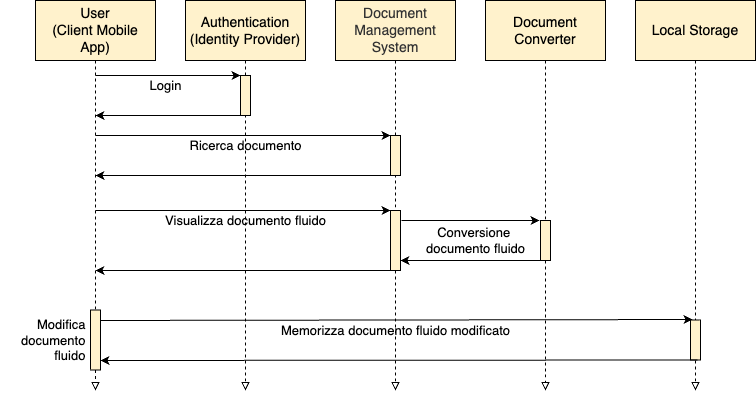
\includegraphics[width=1\textwidth]{img/tesi-2-Use-case2.drawio.png}
                \end{figure}
            \end{column}
            \begin{column}{0.4\textwidth}
                \begin{figure}[H]
                \centering
                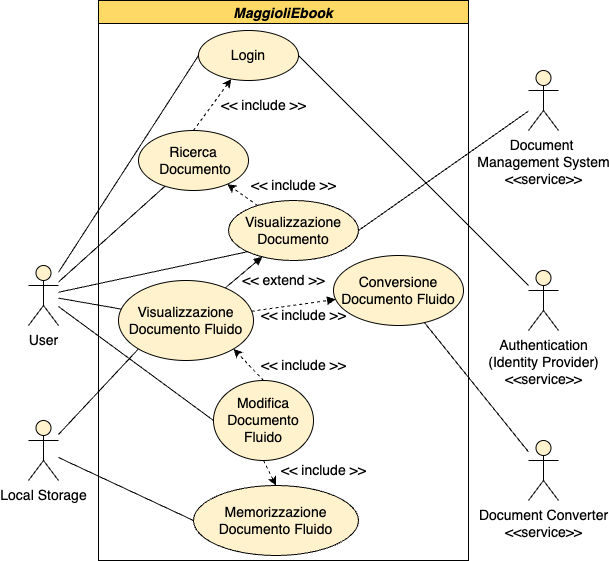
\includegraphics[width=1\textwidth]{img/tesi-1-Use-case.drawio.png}
                \end{figure}
            \end{column}
        \end{columns}
    \end{frame}

    \begin{frame}{Modellazione del dominio}
        \begin{columns}[onlytextwidth]
            \begin{column}{0.45\textwidth}
            \begin{itemize}
                \item Bounded Context:
                    \begin{itemize}
                        \item \textit{Reader} (Core) - Aspetti di maggiore valore per l'utente.
                        \item \textit{Sisred} - Sorgente delle pubblicazioni digitali Maggioli.
                        \item \textit{User} - Gestione delle identità e autenticazione.
                    \end{itemize}
                \item Relazioni Shared Kernel (SK) tra i contesti.
                \end{itemize}
            \end{column}
            \begin{column}{0.55\textwidth}
                \begin{figure}[H]
                \centering
                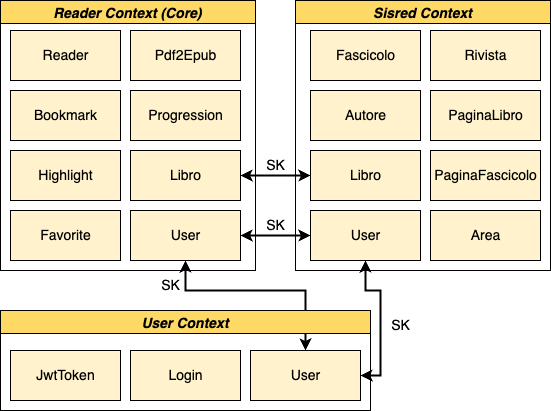
\includegraphics[width=0.9\textwidth]{img/tesi-20-app-domain.drawio.png}
                \end{figure}
            \end{column}
        \end{columns}
    \end{frame}

    \begin{frame}{Clean Architecture}
        \begin{columns}[onlytextwidth]
            \begin{column}{0.45\textwidth}
            \begin{itemize}
                \item Layers:
                    \begin{itemize}
                        \item \textit{Data} - Aggregati di dominio e gestione dati su differenti sorgenti.
                        \item \textit{Domain} - Casi d’uso del sistema che gestiscono il flusso dei dati da o verso il \textit{Data Layer}.
                        \item \textit{View} - UI e gestione eventi provenienti dall’utente o dal sistema.
                    \end{itemize}
                \end{itemize}
            \end{column}
            \begin{column}{0.55\textwidth}
                \begin{figure}[H]
                \centering
                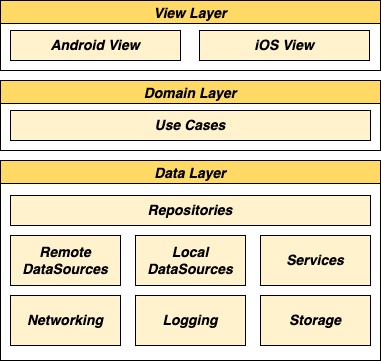
\includegraphics[width=0.8\textwidth]{img/tesi-2-Page-18.drawio.png}
                \end{figure}
            \end{column}
        \end{columns}
    \end{frame}